\title{\textbf{The Automatic Toilet Freshener \\ \large \emph{An technical odyssey}}}

\author{Bastiaan Weijers \\ 3256669 \and Colin Smits \\ 4075390}
\date{}
\documentclass[a4paper, 11pt]{article}
\renewcommand{\familydefault}{\sfdefault}
\usepackage{enumitem}
\usepackage{graphicx}
\usepackage{pdflscape}
\usepackage{hyperref}

\begin{document}
\maketitle

\section{Introduction}


\section{Technical Overview}

%include state diagrams, circuit

\subsection{States}
\label{sub:state}
To start off with the technical details, we need to define states in which are system can be operating. These states must be defined according to the usage of a toilet. So, just after trying out all the circuits with the sensors, we started thinking about distinctive features of a toilet use. 

First of all, you would have to open a door in order to get into the toilet. After that, you would maybe turn on the light in order to see where you are heading, making sure you do not miss the seat and fall down and/or need to clean the floor afterwards. These are the first two point that would suggest the usage of a toilet.

Secondly, you might need to open the lid in order to be able to sit down, or, in the case of a male user, you might need to put the seat up in order to have an increased target area. These are indications of the type of use, while a standing person would not attempt a "Number 2" usage (if you still have a normal functioning brain). Some people might close the lid again after usage, which would indicate they are done using the toilet, setting a time reference for our future system.

After using the toilet, you should be flushing and leaving the area. Therefore, you would open the door (if you did not close it \ldots) and turn off the light (if you actually turned it on \ldots). These are indications of the end of an usage, which would require the freshener to do it's job and clear the area of "bad smells".

\subsection{States of the Sensory}
In \S\hyperref[sub:state]{\ref{sub:state}} we defined the general use case of a toilet system. Now we need to turn these transitions into factors which we can measure using our sensors. 

Starting off with the entrance, we can see that we could place a \textbf{magnetic sensor} in the door opening to measure the state the door is located in. Furthermore, we can measure the amount of light in a room using our \textbf{Light Dependent Resistor} (LDR). A sudden increase of light \emph{might} indicate a person entering the room. You are even more certain when the door is being opened and closed almost simultaneously, but still there is no guarantee. As we will see later on, you can never be sure what a person is doing inside the toilet (\ldots).

As we stated as well, a person might need to open the lid. If we were to place the \textbf{magnetic sensor} on the lid, we might be able to see whether the toilet is being used even more carefully. In order to be able to decide if a person is sitting or standing, we can use the \textbf{distance sensor}. In general, a standing person is further away from the wall behind the toilet then a sitting person.

Using these possible positions we head for the farewell of the toilet for now. We can measure whether a person is gone away from the toilet by using the \textbf{distance sensor} again. After finishing someone might close the lid (\textbf{magnetic sensor}) and walk through the door (\textbf{magnetic sensor} possibly) and turning off the light (\textbf{LDR}). 

\subsection{Decisions, decisions}

We have set out all the possible uses for our sensors. In the end, we decided to do the following placements:
\begin{description}
\item[Distance Sensor] We place the \textit{distance sensor} on the wall behind the toilet to measure the distance between the wall and a person.
\item[Magnetic Sensor] ...
\item[LDR] We locate the \textit{LDR} close to the light source in the toilet to measure the on/off transition of the light.
\end{description}

\noindent After setting the locations, we are able to define our state diagram. However, we still need to make sure that the other components are used as well:
\begin{description}
\item[Temperature sensor] Located somewhere in the toilet just to measure the temperature. Is not used in deciding the states.
\item[Push Buttons] Two of the push buttons will be used for menu control, setting the delay of the spray as well as a reset for the spray counter. The other push button will be the manual override for a spray.
\item[LEDs and LCD Screen] All of these will be used as indicators for states and feedback towards the user.
\end{description}

Our final \hyperref[fig:stateDia]{state diagram} can be seen at the end of the paper.

\section{Development}
\subsection{First circuits}
In order to create a system that is able to do such a difficult task, we had to be able to create the circuits. As we were progressing through all the sensors, one of us hooked up his temperature sensor for testing purposes. It was then that we noticed a smell. The LCD display was not able to tell what it was, because it had no power. We pulled the USB cord from the computer immediately, as the smell was intensifying. After touching the temperature sensor, it became clear that this was the source: it was too hot too handle. This was the first piece which was harmed (but not destroyed), and in the full process of developing, some other pieces would fall victim to bad wiring.

\subsection{The final circuit}
After a week of intense coding and caffeine intake, along with some shocking progress on the circuit, we had created our final circuit without the refresher hooked up yet. We found that our code was fairly able to define our states, so we decided to give it a try. It was then we victimized the second part of our kit: after an hour of trying to get the refresher to work on pin 13, we found that the circuit didn't work, as the led was on, but there was no current going through the refresher. So we decided to replace the parts one by one, only to find out that the MOSFET was not working any more. It was pronounced dead 20th of February, around 6 pm. We then had our circuit fully working, as can be seen in \hyperref[fig:circuit]{this figure}.

To make sure we were able to incorporate all the parts, we have decided to put the push buttons on the analogue inputs as it was fairly easy to code the buttons from there as well. Along with that, we had to put two of the LEDs on the analogue inputs due to lack op space. The decision was made as well to hook the refresher onto pin 13, so that the LED on the Arduino itself would be activated in line with the refresher, so it's easy to see when the refresher is active.

\section{Usage}

\section{Reflection}


%state diagram in landscape mode
\begin{figure}
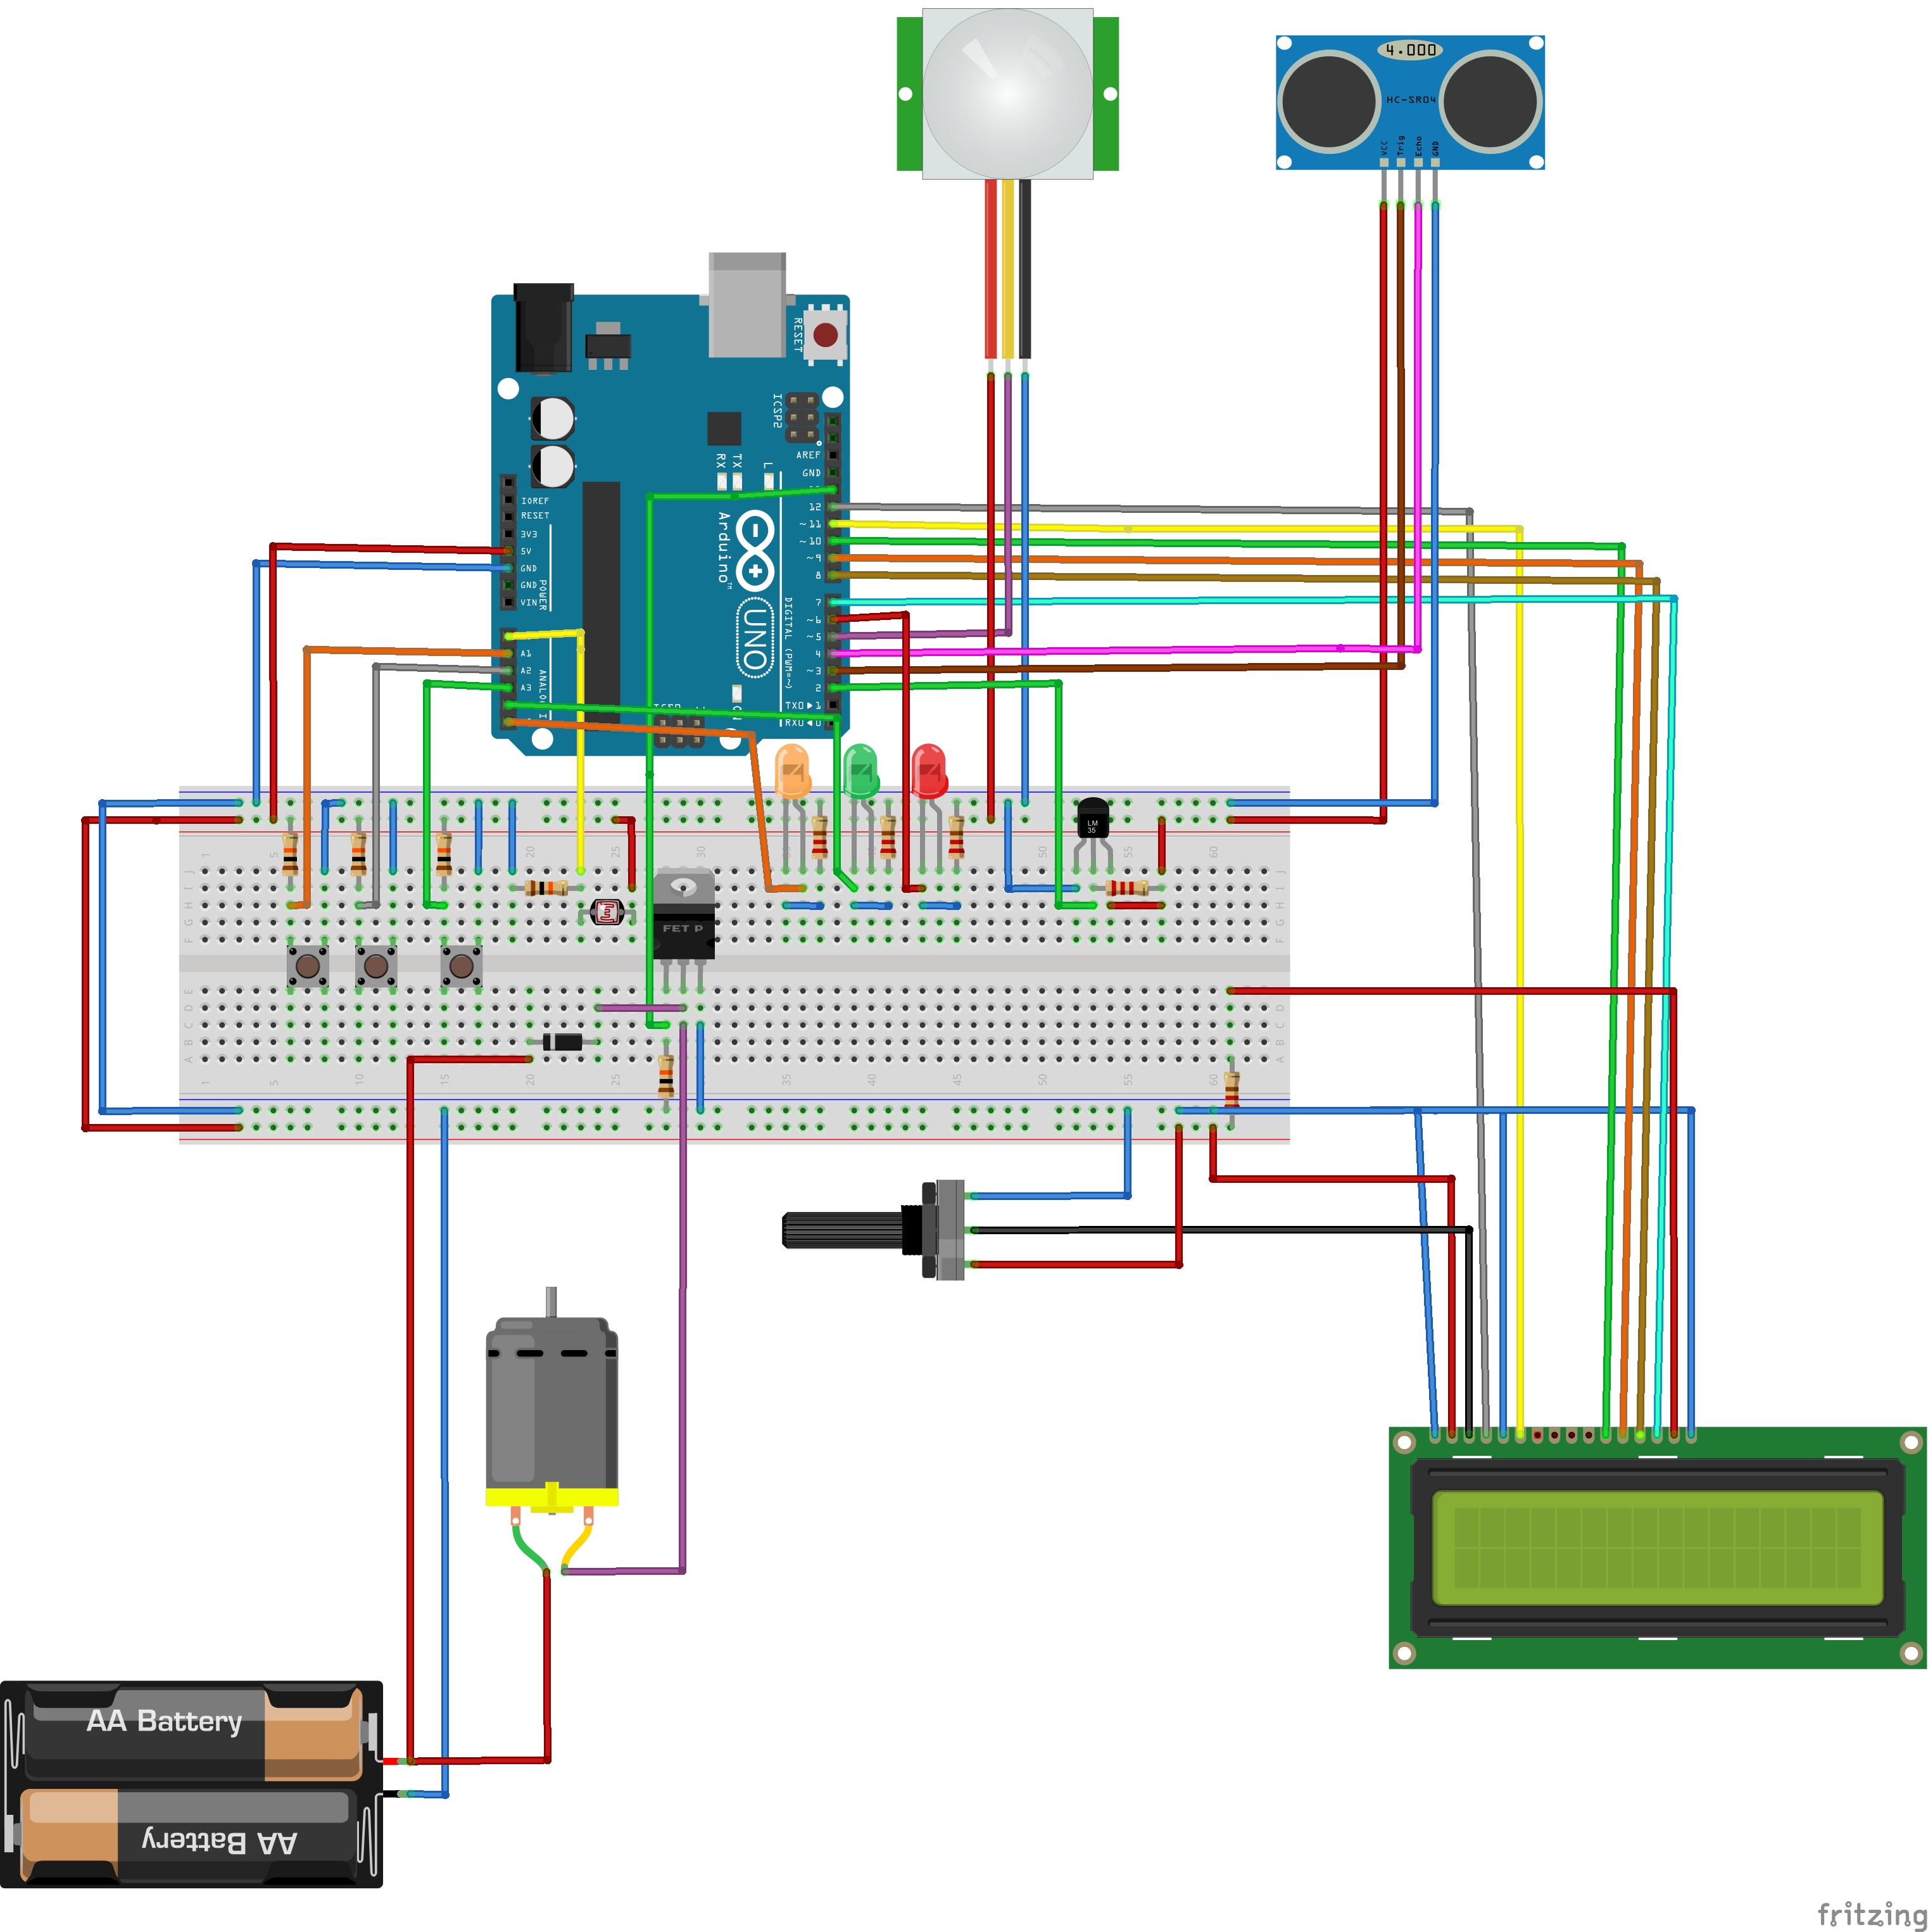
\includegraphics[scale=0.5]{schakeling_bb.png}
\label{fig:circuit}
\caption{The breadboard circuit of our system}
\end{figure}  
\newpage
\begin{landscape}
\begin{figure}[h!]
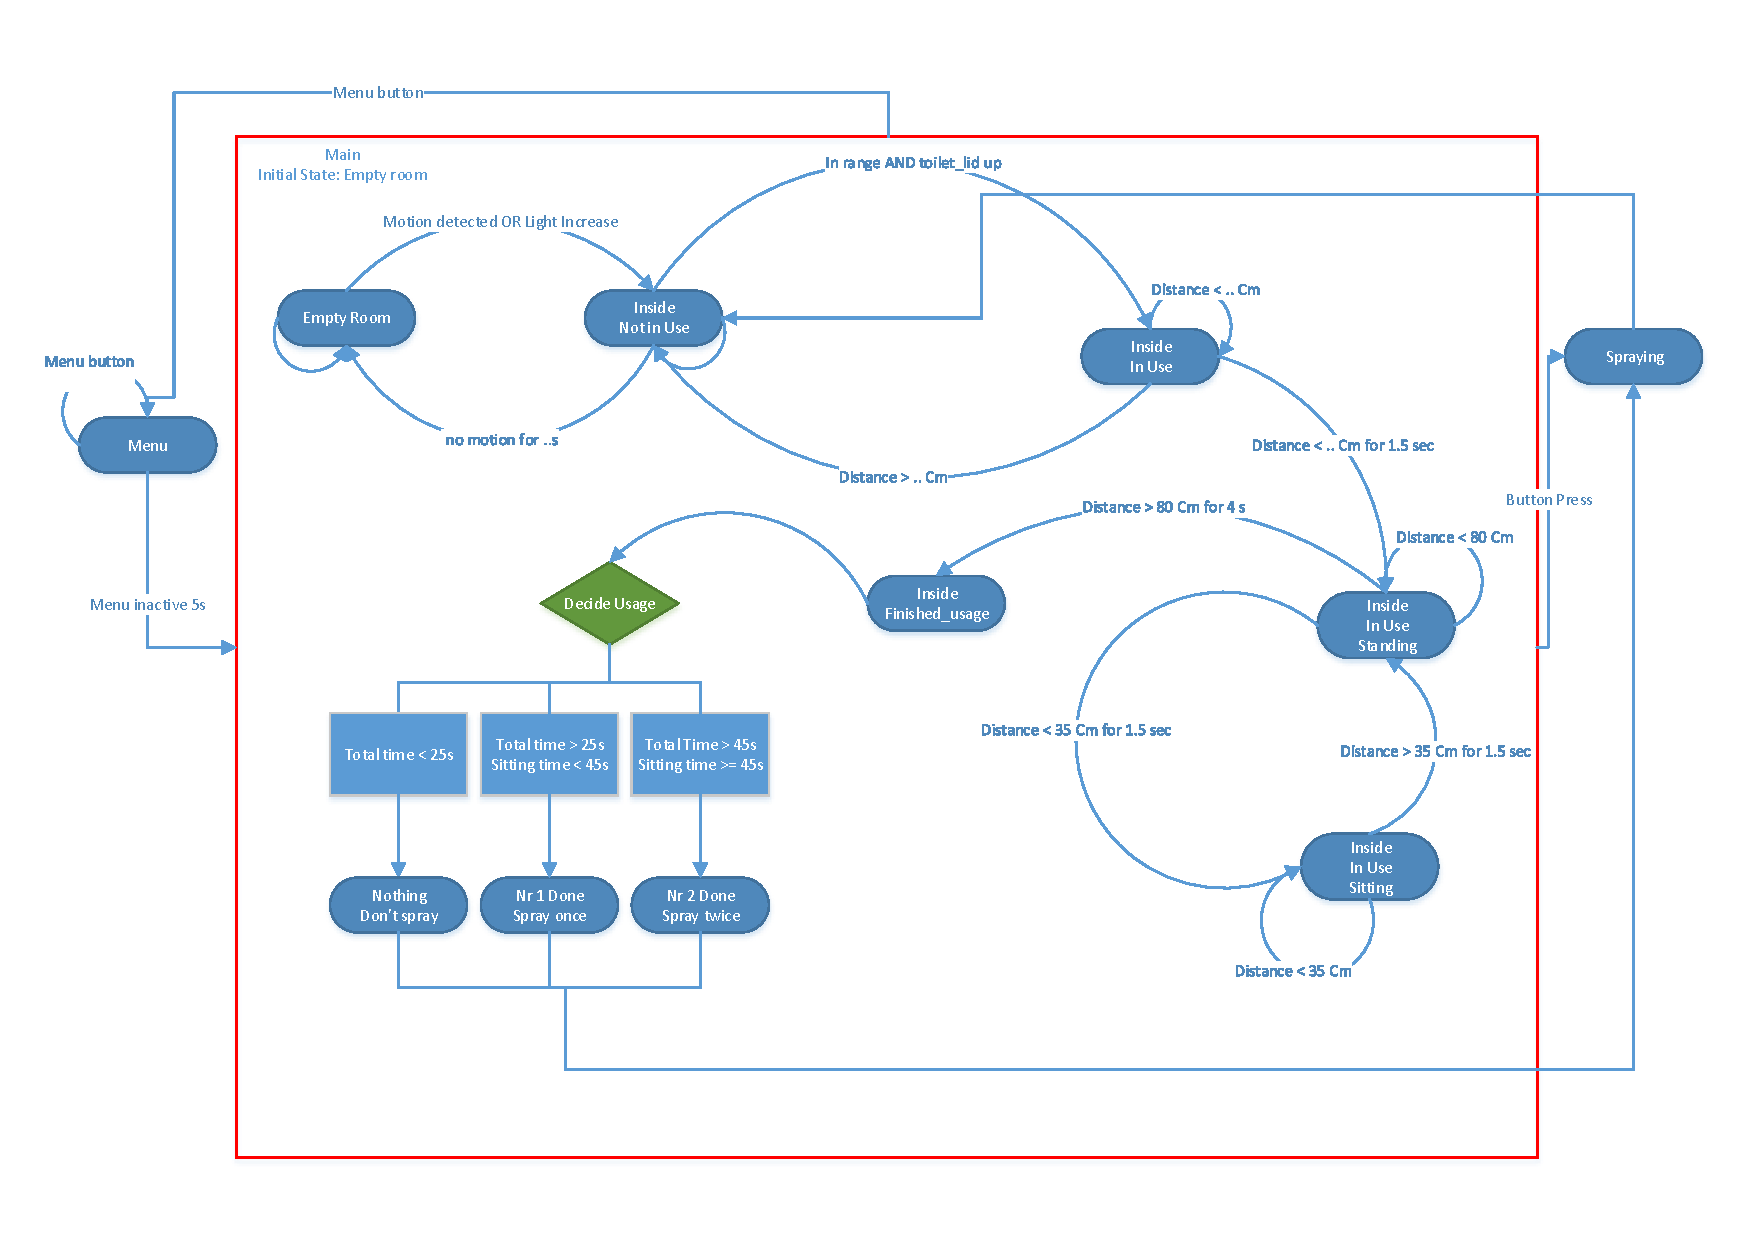
\includegraphics[scale=0.7]{State_Diagram.pdf}
\label{fig:stateDia}
\caption{State Diagram of our system}
\end{figure}
\end{landscape}



\end{document}
